%  A simple AAU report template.
%  2015-05-08 v. 1.2.0
%  Copyright 2010-2015 by Jesper Kjær Nielsen <jkn@es.aau.dk>
%
%  This is free software: you can redistribute it and/or modify
%  it under the terms of the GNU General Public License as published by
%  the Free Software Foundation, either version 3 of the License, or
%  (at your option) any later version.
%
%  This is distributed in the hope that it will be useful,
%  but WITHOUT ANY WARRANTY; without even the implied warranty of
%  MERCHANTABILITY or FITNESS FOR A PARTICULAR PURPOSE.  See the
%  GNU General Public License for more details.
%
%  You can find the GNU General Public License at <http://www.gnu.org/licenses/>.


%  2015-05-08 v. 1.2.0
%  Copyright 2010-2015 by Jesper Kjær Nielsen <jkn@es.aau.dk>
%
%  This is free software: you can redistribute it and/or modify
%  it under the terms of the GNU General Public License as published by
%  the Free Software Foundation, either version 3 of the License, or
%  (at your option) any later version.
%
%  This is distributed in the hope that it will be useful,
%  but WITHOUT ANY WARRANTY; without even the implied warranty of
%  MERCHANTABILITY or FITNESS FOR A PARTICULAR PURPOSE.  See the
%  GNU General Public License for more details.
%
%  You can find the GNU General Public License at <http://www.gnu.org/licenses/>.
%
\documentclass[11pt,oneside,a4paper,openany]{report}
%%%%%%%%%%%%%%%%%%%%%%%%%%%%%%%%%%%%%%%%%%%%%%%%
% Language, Encoding and Fonts
% http://en.wikibooks.org/wiki/LaTeX/Internationalization
%%%%%%%%%%%%%%%%%%%%%%%%%%%%%%%%%%%%%%%%%%%%%%%%
% Select encoding of your inputs. Depends on
% your operating system and its default input
% encoding. Typically, you should use
%   Linux  : utf8 (most modern Linux distributions)
%            latin1 
%   Windows: ansinew
%            latin1 (works in most cases)
%   Mac    : applemac
% Notice that you can manually change the input
% encoding of your files by selecting "save as"
% an select the desired input encoding. 
\usepackage[utf8]{inputenc}
% Make latex understand and use the typographic
% rules of the language used in the document.
\usepackage[danish,english]{babel}
% Use the palatino font
\usepackage[sc]{mathpazo}
\linespread{1.05}         % Palatino needs more leading (space between lines)
% Choose the font encoding
\usepackage[T1]{fontenc}
%%%%%%%%%%%%%%%%%%%%%%%%%%%%%%%%%%%%%%%%%%%%%%%%
% Graphics and Tables
% http://en.wikibooks.org/wiki/LaTeX/Importing_Graphics
% http://en.wikibooks.org/wiki/LaTeX/Tables
% http://en.wikibooks.org/wiki/LaTeX/Colors
%%%%%%%%%%%%%%%%%%%%%%%%%%%%%%%%%%%%%%%%%%%%%%%%
% load a colour package
\usepackage[table]{xcolor}
\definecolor{aaublue}{RGB}{33,26,82}% dark blue
% The standard graphics inclusion package
\usepackage{graphicx}
% Set up how figure and table captions are displayed
\usepackage{caption}
\captionsetup{%
  font=footnotesize,% set font size to footnotesize
  labelfont=bf % bold label (e.g., Figure 3.2) font
}
% Make the standard latex tables look so much better
\usepackage{array,booktabs}
% Enable the use of frames around, e.g., theorems
% The framed package is used in the example environment
\usepackage{framed}

%%%%%%%%%%%%%%%%%%%%%%%%%%%%%%%%%%%%%%%%%%%%%%%%
% Mathematics
% http://en.wikibooks.org/wiki/LaTeX/Mathematics
%%%%%%%%%%%%%%%%%%%%%%%%%%%%%%%%%%%%%%%%%%%%%%%%
% Defines new environments such as equation,
% align and split 
\usepackage{amsmath}
% Adds new math symbols
\usepackage{amssymb}
% Use theorems in your document
% The ntheorem package is also used for the example environment
% When using thmmarks, amsmath must be an option as well. Otherwise \eqref doesn't work anymore.
\usepackage[framed,amsmath,thmmarks]{ntheorem}

%%%%%%%%%%%%%%%%%%%%%%%%%%%%%%%%%%%%%%%%%%%%%%%%
% Page Layout
% http://en.wikibooks.org/wiki/LaTeX/Page_Layout
%%%%%%%%%%%%%%%%%%%%%%%%%%%%%%%%%%%%%%%%%%%%%%%%
% Change margins, papersize, etc of the document
\usepackage[
  inner=28mm,% left margin on an odd page
  outer=41mm,% right margin on an odd page
  ]{geometry}
% Modify how \chapter, \section, etc. look
% The titlesec package is very configureable
\usepackage{titlesec}
\titleformat{\chapter}[display]{\normalfont\huge\bfseries}{\chaptertitlename\ \thechapter}{20pt}{\Huge}
\titleformat*{\section}{\normalfont\Large\bfseries}
\titleformat*{\subsection}{\normalfont\large\bfseries}
\titleformat*{\subsubsection}{\normalfont\normalsize\bfseries}
%\titleformat*{\paragraph}{\normalfont\normalsize\bfseries}
%\titleformat*{\subparagraph}{\normalfont\normalsize\bfseries}

% Clear empty pages between chapters
\let\origdoublepage\cleardoublepage
\newcommand{\clearemptydoublepage}{%
  \clearpage
  {\pagestyle{empty}\origdoublepage}%
}
\let\cleardoublepage\clearemptydoublepage

% Change the headers and footers
\usepackage{fancyhdr}
\pagestyle{fancy}
\fancyhf{} %delete everything
\renewcommand{\headrulewidth}{0pt} %remove the horizontal line in the header
\fancyhead[RE]{\small\nouppercase\leftmark} %even page - chapter title
\fancyhead[LO]{\small\nouppercase\rightmark} %uneven page - section title
\fancyhead[LE,RO]{\thepage} %page number on all pages
% Do not stretch the content of a page. Instead,
% insert white space at the bottom of the page
\raggedbottom
% Enable arithmetics with length. Useful when
% typesetting the layout.
\usepackage{calc}

%%%%%%%%%%%%%%%%%%%%%%%%%%%%%%%%%%%%%%%%%%%%%%%%
% Bibliography
% http://en.wikibooks.org/wiki/LaTeX/Bibliography_Management
%%%%%%%%%%%%%%%%%%%%%%%%%%%%%%%%%%%%%%%%%%%%%%%%
%\usepackage[backend=bibtex,
%  bibencoding=utf8
%  ]{biblatex}
%\addbibresource{references}

%%%%%%%%%%%%%%%%%%%%%%%%%%%%%%%%%%%%%%%%%%%%%%%%
% Misc
%%%%%%%%%%%%%%%%%%%%%%%%%%%%%%%%%%%%%%%%%%%%%%%%
% Add bibliography and index to the table of
% contents
%\usepackage[nottoc]{tocbibind}
% Add the command \pageref{LastPage} which refers to the
% page number of the last page
\usepackage{lastpage}
% Add todo notes in the margin of the document
\usepackage[
%  disable, %turn off todonotes
  colorinlistoftodos, %enable a coloured square in the list of todos
  textwidth=\marginparwidth, %set the width of the todonotes
  textsize=scriptsize, %size of the text in the todonotes
  ]{todonotes}
\usepackage[tocindentauto]{tocstyle}
\usepackage[super]{nth}

%%%%%%%%%%%%%%%%%%%%%%%%%%%%%%%%%%%%%%%%%%%%%%%%
% Hyperlinks
% http://en.wikibooks.org/wiki/LaTeX/Hyperlinks
%%%%%%%%%%%%%%%%%%%%%%%%%%%%%%%%%%%%%%%%%%%%%%%%
% Enable hyperlinks and insert info into the pdf
% file. Hypperref should be loaded as one of the 
% last packages
\usepackage{hyperref}
\hypersetup{%
	pdfpagelabels=true,%
	plainpages=false,%
	pdfauthor={Author(s)},%
	pdftitle={Title},%
	pdfsubject={Subject},%
	bookmarksnumbered=true,%
	colorlinks=false,%
	citecolor=black,%
	filecolor=black,%
	linkcolor=black,% you should probably change this to black before printing
	urlcolor=black,%
	pdfstartview=FitH%
}
\usepackage{tabularx}
\usepackage{makecell}

% Draft watermark
%\usepackage{draftwatermark}
%\SetWatermarkText{DRAFT}
% package inclusion and set up of the document
% see, e.g., http://en.wikibooks.org/wiki/LaTeX/Formatting#Hyphenation
% for more information on word hyphenation
\hyphenation{ex-am-ple hy-phen-a-tion short}
\hyphenation{long la-tex}% 
%  A simple AAU report template.
%  2015-05-08 v. 1.2.0
%  Copyright 2010-2015 by Jesper Kjær Nielsen <jkn@es.aau.dk>
%
%  This is free software: you can redistribute it and/or modify
%  it under the terms of the GNU General Public License as published by
%  the Free Software Foundation, either version 3 of the License, or
%  (at your option) any later version.
%
%  This is distributed in the hope that it will be useful,
%  but WITHOUT ANY WARRANTY; without even the implied warranty of
%  MERCHANTABILITY or FITNESS FOR A PARTICULAR PURPOSE.  See the
%  GNU General Public License for more details.
%
%  You can find the GNU General Public License at <http://www.gnu.org/licenses/>.
%
%
%
% see, e.g., http://en.wikibooks.org/wiki/LaTeX/Customizing_LaTeX#New_commands
% for more information on how to create macros

%%%%%%%%%%%%%%%%%%%%%%%%%%%%%%%%%%%%%%%%%%%%%%%%
% Macros for the titlepage
%%%%%%%%%%%%%%%%%%%%%%%%%%%%%%%%%%%%%%%%%%%%%%%%
%Creates the aau titlepage
\newcommand{\aautitlepage}[2]{%
  {
    %set up various length
    \ifx\titlepageleftcolumnwidth\undefined
      \newlength{\titlepageleftcolumnwidth}
      \newlength{\titlepagerightcolumnwidth}
    \fi
    \setlength{\titlepageleftcolumnwidth}{0.5\textwidth-\tabcolsep}
    \setlength{\titlepagerightcolumnwidth}{\textwidth-2\tabcolsep-\titlepageleftcolumnwidth}
    %create title page
    \thispagestyle{empty}
    \noindent%
    \begin{tabular}{@{}ll@{}}
      \parbox{\titlepageleftcolumnwidth}{
        
\includegraphics[width=\titlepageleftcolumnwidth]{figs/apl_small_vertical_blue.pdf}
      } &
      \parbox{\titlepagerightcolumnwidth}{\raggedleft\sf\small
        #2
      }\bigskip\\
       #1 &
      \parbox[t]{\titlepagerightcolumnwidth}{%
      }\\
    \end{tabular}
    \clearpage
  }
}

%Create english project info
\newcommand{\englishprojectinfo}[4]{%
  \parbox[t]{\titlepageleftcolumnwidth}{
    \textbf{Title:}\\ #1\bigskip\par
    \textbf{Project Participants:}\\ #2\bigskip\par
    \textbf{Authors:}\\ #3\bigskip\par
    \textbf{Date:}\\ #4
  }
}


%%%%%%%%%%%%%%%%%%%%%%%%%%%%%%%%%%%%%%%%%%%%%%%%
% An example environment
%%%%%%%%%%%%%%%%%%%%%%%%%%%%%%%%%%%%%%%%%%%%%%%%
\theoremheaderfont{\normalfont\bfseries}
\theorembodyfont{\normalfont}
\theoremstyle{break}
\def\theoremframecommand{{\color{gray!50}\vrule width 5pt \hspace{5pt}}}
\newshadedtheorem{exa}{Example}[chapter]
\newenvironment{example}[1]{%
		\begin{exa}[#1]
}{%
		\end{exa}
}
% my new macros

\usepackage{xspace}
\usepackage{times}
\usepackage{epsfig}
\usepackage{graphicx}
\usepackage{amsmath}
\usepackage{amssymb}
\usepackage{booktabs}
\usepackage{paralist}
\usepackage{textcase}
\usepackage{float}
\usepackage{subcaption}
\usepackage{stackengine}

\newcommand{\figref}[1]{Figure~\ref{#1}}
\newcommand{\secref}[1]{Section~\ref{#1}}

\newcommand{\eg}{e.g.,\xspace}
\newcommand{\APL}{JHU/APL\xspace}
\newcommand*\rot{\rotatebox{90}}

\newcommand{\subsubheaderbf}[1]{\mbox{\textbf{#1}\hspace*{2.5mm}}}
\newcommand{\subsubheaderit}[1]{\mbox{\textit{#1}\hspace*{2.5mm}}}
\newcommand{\subsubheadertt}[1]{\mbox{\texttt{#1}\hspace*{2.5mm}}}
\newcommand{\subsubheader}[1]{\mbox{#1\hspace*{2.5mm}}}

\begin{document}
%frontmatter
\pagestyle{empty} %disable headers and footers
\pagenumbering{roman} %use roman page numbering in the frontmatter
\pdfbookmark[0]{Title}{label:titlepage_en}
\aautitlepage{%
  \englishprojectinfo{
    Lifelong Learning Machines \\ Metrics Framework \& \\ Proposed Metrics
  }{%
  	\APL Test \& Evaluation Team
  }{%
    Megan Baker \\
    Gautam Vallabha \\ 
  }{%
    \today % date of completion
  }%
}{%department and address
  \textbf{\APL}\\
  \href{http://www.jhuapl.edu/}{http://www.jhuapl.edu/}
}

\cleardoublepage
\pdfbookmark[0]{Contents}{label:contents}
\pagestyle{fancy} %enable headers and footers again
\tableofcontents
%mainmatter
\pagenumbering{arabic} %use arabic page numbering in the mainmatter
\chapter{Introduction}\label{ch:overview}
A crucial part of the T\&E Framework (TEF) is to log information during the operation of a lifelong learning system and use this to derive \textit{metrics of lifelong learning}, i.e., to characterize how well the system learns along the dimensions (Core Capabilities) set out in the DARPA L2M BAA, such as Continual Learning (CL) and Adaptation to New Tasks (ANT). This is termed the \textbf{Metrics Framework}.\\[0.2in]

\begin{figure}[h]
	\centering
	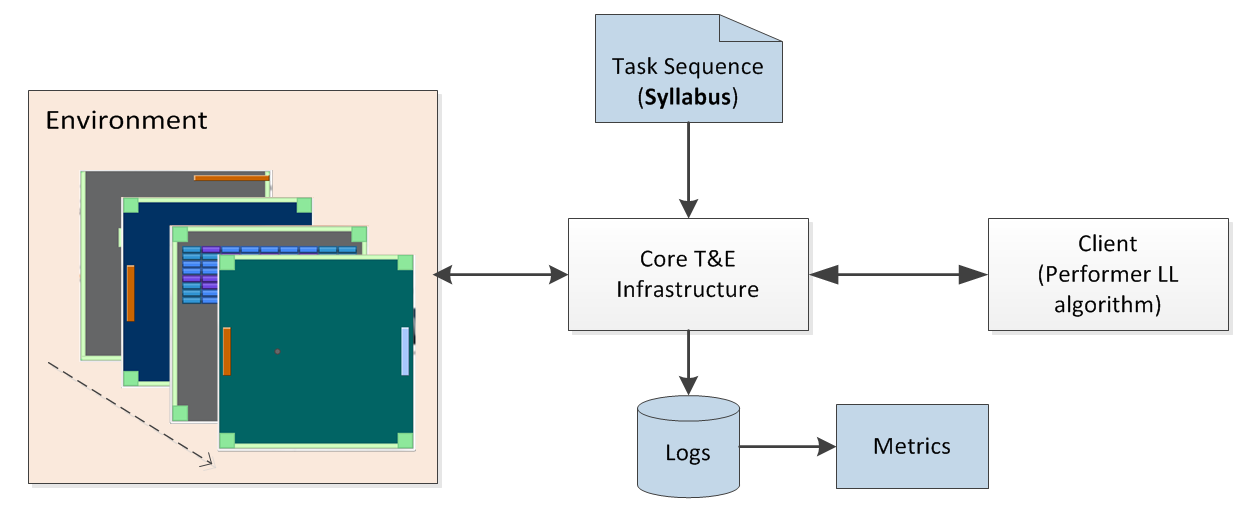
\includegraphics[width=0.8\columnwidth]{sections/figs/metrics_diagram.png}
	\caption{Depiction of the Metrics Framework}
	\label{fig:framework}
\end{figure}

\flushleft The Metrics Framework consists of three components:\\[0.2in]
\begin{enumerate}
\item \textit{Performance Logging.} As a learning algorithm goes through a syllabus, Learnkit automatically logs information about the performance of the learning algorithm. For Agent learning, the logged information consists of the total reward for each episode; for classification learning, the logged information consists of the performance error on each batch (the definition of “performance error” is task-specific).\\[0.1in]
\item \textit{Metrics Calculation.} After the training is completed, the performance logs are read and processed by a separate L2M Python package. This package (the l2metrics repository) consists of a set of predefined metrics, and a Python class hierarchy for extending the predefined set with custom metrics.\\[0.1in]
\item \textit{Syllabus Annotation.} The metrics calculation assumes that the Learnkit syllabus has specific annotations (e.g., to distinguish training vs. test phases, or different parts of a test phase); relatedly, different syllabi may exercise different aspects of lifelong learning, such as Continual Learning versus Adapting to New Tasks. Consequently, authoring correctly-annotated syllabi is a crucial component of the Metrics Framework.\\[0.2in]
\end{enumerate}
    
The following table summarizes the different ways in which we anticipate performers will engage with the Metrics Framework. 

\begin{table}[h]
\begin{tabular}{|l|l|}
\hline
\textbf{Goal:}                                                                              & \textbf{Relevant Section:} \\ \hline
\begin{tabular}[c]{@{}l@{}}Generate metrics for a syllabus. Run an L2 algorithm\\ using a predefined syllabus, run the predefined metrics,\\ and view the results\end{tabular} & 3. Generating Metrics for a Syllabus\\\hline                                                                              
\begin{tabular}[c]{@{}l@{}}Create a custom syllabus. Run an L2 algorithm with a\\custom syllabus, and run predefined metrics.\end{tabular} & 4. Creating Custom Syllabi\\\hline         
\begin{tabular}[c]{@{}l@{}}Create a custom metric. Run an L2 algorithm with a\\predefined or custom syllabus, and run a custom metric.\end{tabular} & \begin{tabular}[c]{@{}l@{}}4. Creating Custom Syllabi\\5. Creating Custom Metrics\end{tabular}\\ \hline
                                                                                  
\end{tabular}
\end{table}

\section{Conceptual Overview}

\subsection*{Agent Learning}

The T\&E Framework uses the information contained in an annotated syllabusto produce a sequence of specific tasks, known as episodes, for an agent learner and automaticallly generates the performance logs from which metrics will be calculated. Figure~\ref{fig:workflow} depicts the workflow of the system as described below.\\[0.2in]

\begin{figure}[h]
	\centering
	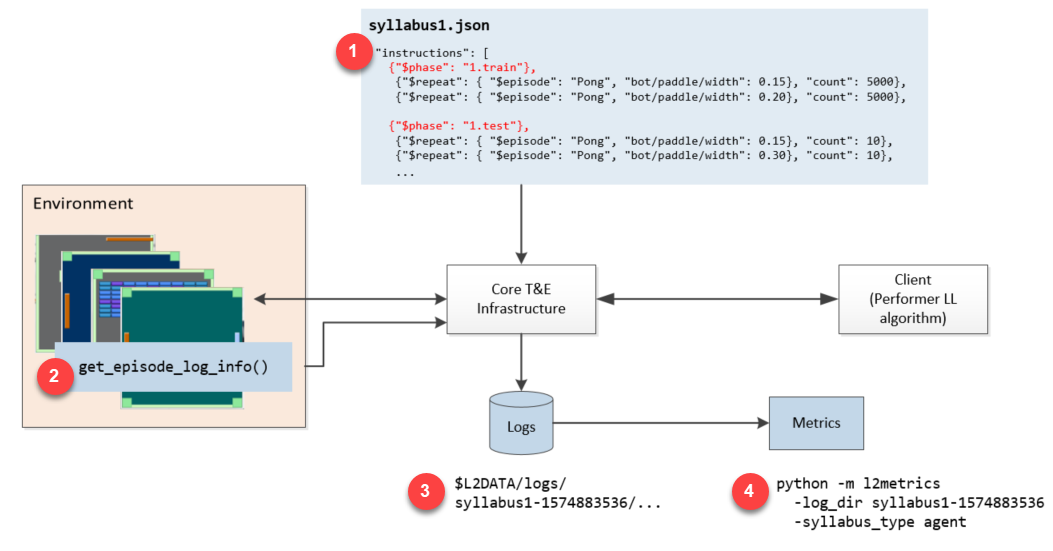
\includegraphics[width=0.9\columnwidth]{sections/figs/metrics_overview_1.png}
	\caption{Workflow in the Metrics Framework}
	\label{fig:workflow}
\end{figure}

\begin{enumerate}
\item The performance logging starts with an annotated syllabus (see Figure~\ref{fig:annotated_syllabus} for an example). The annotation consists of the “\$phase” instructions; the phase values (e.g., “1.train”) have a specific structure that is used during the metrics calculation.\\[0.4in]

\begin{figure}[h]
	\centering
	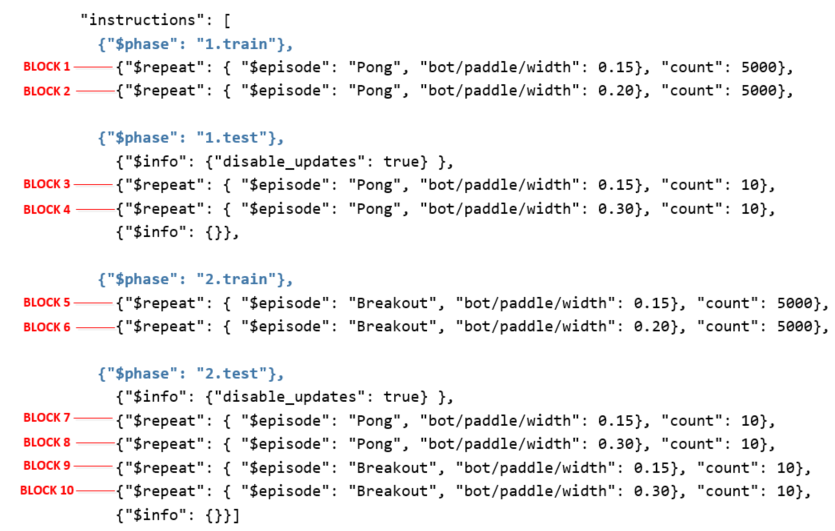
\includegraphics[width=0.8\columnwidth]{sections/figs/syllabus_annotated_blocks.png}
	\caption{An Annotated Syllabus Example}
	\label{fig:annotated_syllabus}
\end{figure}


\item Tasks in the L2M environment (such as Pong L2Arcade, or L2StarCraft CollectThings) have a special method (
\begin{small}
\verb|get_episode_log_info| 
\end{small}
) that reports the total reward and related performance information for each episode. This is automatically called by Learnkit as the syllabus is processed; performer code does not need to do anything (and in particular, the performer algorithm should not call 
\begin{small}
\verb|get_episode_log_info| 
\end{small}
or use the information reported therein).\\[0.1in]

\item The performance logs from running the syllabus are automatically saved under the L2M logging directory (the default value of the top-level logging directory is OS-specific, and it can be overridden using the \$L2DATA environment variable). The logs for running a specific syllabus are saved under a unique directory name <syllabus\_name>-<timestamp>.The
\begin{small}
\verb|python -m learnkit.info|
\end{small}
command shows the location of the directory, along with the most recently created log directory:\\[0.1in]

\begin{small}
\begin{verbatim}
bakermm1@bakermm1-ll2:~/L2M/l2metrics$ python -m learnkit.info
Learnkit v0.5.0
L2 data folder:
   /home/bakermm1/l2data
L2 logs folder:
   /home/bakermm1/l2data/logs
Most recent log folder:
   /home/bakermm1/l2data/logs/syllabus_CL-1575473425723
   created on 2019-12-04T10:30:25
\end{verbatim}
\end{small}

Under \$L2DATA/logs/<syllabus\_name>-<timestamp>/ the directory tree looks like this: <worker\_id>/<phase\_name>/<task\_name>/{block-report, data-log}.tsv. A few points worth noting about this logging structure:\\[0.2in]
\begin{itemize}
\item The worker ID is for distributed training. The ordering of episodes is maintained across workers, so an episode number is unique across the distributed training.\\[0.1in]
\item The syllabus is notionally divided into a sequence of blocks; each block is a sequence of episodes with the same Task name and parameter values. See Figure~\ref{fig:annotated_syllabus} for an example.\\[0.1in]
\item Each episode consists of one or more sub-episodes (each sub-episode is a reset, followed by one or more steps). This is the granularity for the performance logging – for each sub-episode, the logs record the total reward and whether that sub-episode as complete (i.e., continued until done) or incomplete. \\[0.1in]
\item block-report.tsv contains metadata about each block. data-log.tsv contains the actual logged information about each episode and its sub-episodes. Note that in the logs, “task” and “sub\_task” specify the episode and sub-episode number, respectively.\\[0.1in]
\end{itemize}
\item Once the learning algorithm is done, the predefined metrics calculations can be invoked by specifying the directory of the log files, e.g.: \\[0.1in]
\end{enumerate}

\begin{small}
\begin{verbatim} python -m l2metrics  -log_dir syllabus1-1574883536 -syllabus_type agent \end{verbatim}
\end{small}

Conceptually, the above command loads the log data into a single data table, hands it to each Metric (a Python class), collects the results and prints them out. It is also possible to write a custom script with custom metrics and with full control over which metrics are calculated.

\subsection*{Classification Learning}

The logging for classification learning is conceptually similar to that for agent learning. The main difference is in what gets logged and at what granularity (corresponding to Workflow steps 2 and 3 in Figure~\ref{fig:framework}).\\[0.1in]

Recall that a Classification syllabus consists of a sequence of datasets; each dataset consists of one or batches; each batch is a sequence of examples; each example is one input to the learning agent, with an optional output or ground truth value. When performer code interacts a Classification Task (such as CIFAR100), the code looks something like this:

\begin{small}
\begin{verbatim} 
for dataset in syllabus.datasets():       
       dataset.reset()
       done = False
       while not done:
           batch, done, info = dataset.next_batch()
           y_hat = do_inference(batch['inputs'])  # performer code
           y = dataset.get_labels(batch[id'], y_hat)
           if y:
               calculate_loss_and_update_model(y, y_hat)  # performer code 
\end{verbatim}
\end{small}

Crucially, the performer code has to submit the estimated outputs
\begin{small}
\verb|y_hat|
\end{small}via the
\begin{small}
\verb|get_labels|
\end{small}method; this is done for both training and test data. The Classification Task uses this
\begin{small}
\verb|y_hat|
\end{small}to calculate the error for the batch, and has a special method
\begin{small}
\verb|get_batch_log_info|
\end{small}that reports the error information to Learnkit for logging. This method is automatically called by Learnkit as the syllabus is processed; performer code does not need to do anything, and in particular should not invoke
\begin{small}
\verb|get_batch_log_info.|
\end{small}This information is only intended for Learnkit logging; performers should use their own loss functions as appropriate for their models.

\section{Sample Workflow to Generate Metrics}

The following instuctions illustrate how to operate in the Metrics Framework in a sample environment called Minigrid. Please note that while we have adapted this environment to work with Learnkit, it will not be used for the T\&E Framework but serves as a quick-to-train example to generate log files in the proper format. After setting up the python packages (steps 1-3), an agent should be trained using the minigridkit script (step 4). Behind the scenes, this script uses Learnkit to load a Continual Learning syllabus which queues up sequences of episodes in which the agent can learn. While the agent is being fed these episodes, Learnkit automatically logs the reward achieved at the end of each episode and saves it to TSV files. The location of these files must be passed (step 5) to the l2metrics code, which computes Metrics and prints out the results (step 6). \\[0.2in]

\begin{enumerate}

\item Clone the learnkit repository\\
\begin{small}
\verb|pip install -e learnkit\|\\[0.1in]
\end{small}

\item Clone the minigridkit repository\\
\begin{small}
\verb|pip install -e minigridkit\|\\[0.1in]
\end{small}

\item Clone the l2metrics repository\\
\begin{small}
\verb|pip install -e l2metrics\|\\[0.1in]
\end{small}

\item Train an agent in the Minigrid environment. This will take a few minutes. When it starts you should see an INFO level message showing the top level directory where logs are being written.\\[0.1in]
\begin{small}
\verb|python minigrid_learnkit/examples/minigrid_train_ppo.py| \\
\verb|2019-12-04 10:30:25,723 <22980> | \\
\verb|[INFO    ] root - Logging to: /home/bakermm1/l2data/logs|\\[0.1in]
\end{small}

\item Store the last used logging directory in a temporary variable.\\
\begin{small}
\verb|log_dir =$(ls -t -1 `python -m learnkit.info -get logdir`| |\verb| head -1)|\\[0.1in]
\end{small}
\item Pass the variable just set as the 
\begin{small}
\verb|-log_dir|
\end{small}parameter when you run calc\_metrics\\
\begin{small}
\verb|cd l2metrics/examples|
\verb|python calc_metrics.py -syllabus_subtype=CL -log_dir=$log_dir|\\[0.2in]
\end{small}
\end{enumerate}
The output should print to the screen and should look something like this:\\[0.2in]

\begin{verbatim}

Metric: Average Within Block Saturation Calculation

Averaged Value: {'global_within_block_saturation': 0.875959925753812, 
                'global_num_eps_to_saturation': 197.45454545454547}
                
Per Block Values: {
'saturation_value': {0: 0.8488624196510561, 1: 0.822495598845599, 
2: 0.8413838383838385, 3: 0.9651983081298474, 4: 0.8791413586413588, 
5: 0.8132655122655124, 6: 0.8654549980322708, 7: 0.9549258642961517, 
8: 0.9681967251617378, 9: 0.8410522366522368, 10: 0.8355823232323233},

'eps_to_saturation': {0: 185, 1: 30, 2: 81, 3: 107, 4: 610, 5: 83, 
6: 84, 7: 100, 8: 739, 9: 103, 10: 50}}

Metric: An Example Custom Metric
Averaged Value: {'global_perf': 0.9217597535934293}
Per Block Values: {'global_perf': 0.9217597535934293}

Process finished with exit code 0

\end{verbatim}

\chapter{Syllabus Design}\label{ch:syllabus_design}

With the Core Capabilties in mind, we move on to intentional design of the syllabi. As a reminder, the calculation of these metrics seeks to answer a question that may differ from traditional reinforcement learning evaluation criteria, and thus, we enforce a semi-rigid structure to these evaluation tasks.

\section{Conceptual Model}

\section{An Example Syllabus}
    
\section{Proposed Metrics by Core Capability}

\section{Design Your Own Syllabus}

\subsection*{Continual Learning} 
\textit{Syllabus Structure Requirements}\\
\noindent\rule{8cm}{0.4pt}
\flushleft 1. This syllabus consists of a single task with parametric variations\\
\textit{Can involve interpolation of parameters, noisy parameters, etc. but has only one task \\}


\flushleft 2. Each phase consists of a training and optional but recommended evaluation block\\
\textit{Training block is training on one or more parametric variations \\}
\noindent\rule{8cm}{0.4pt}

\flushleft\textit{Metric Evaluation Questions}\\[0.1in]

Note that some of these are computed as a basis for comparison for future eval blocks, etc.\\[0.1in]

\textbf{Question:} What level of performance does the agent achieve during training?\\
\textit{Metric:} Saturation Value\\[0.1in]


\textbf{Question:} How quickly does it achieve this saturation value?\\
\textit{Metric:} Time to Saturation\\[0.1in]

\textbf{Question:} How quickly does an agent learn during training?\\
\textit{Metric:} Normalized Integral of Reward/Time\\[0.1in]


\textbf{Question:} Can the agent adjust to changes in the environment? How quickly does it recover?\\
\textit{Metric:} Recovery Time\\[0.1in]


\textbf{Question:} Can the agent maintain performance on previously learned parameters after being trained with new ones?\\
\textit{Metric:} Performance Maintenance\\[0.1in]


\textbf{Question:} How does the lifelong learning agent's performance compare to a traditional agent?\\
\textit{Metric:} Performance relative to STE \\[0.2in]
            
            

After these metrics are computed, the agent will receive a score for  each of these metrics for a Continual Learning syllabus, which will be aggregated to form its Continual Learning score. For now, an average of the scores achieved is reported in each phase/block, but more sophisticated methods may replace these in the future. See below for more details; more information is on its way.
    


\subsection*{Formal Metric Definitions}

\textbf{1. Saturation Value}\\
Purpose: The saturation value is computed to quantify the maximum maintained value by the agent.\\
Calculated by: Since multiple rewards may be logged per episode, the mean is taken per episode. Then, the max of the rolling average is taken of the mean reward per episode with a smoothing parameter, s (default, 0.1)\\
Compared to: Future or single task expert saturation values of the same task\\[0.1in]         


\textbf{2. Time to Saturation}\\
Purpose: Time to saturation is used to quantify how quickly, in number of episodes, the agent took to achieve the saturation value computed above.\\
Calculated by: The first time the saturation value (or above) is seen, that episode number is recorded\\
Compared to: Future times to saturation of the same task\\[0.1in]


\textbf{3. Normalized Integral of Reward/Time}\\
Purpose: Taking the Integral of Accumulated Reward over Time allows for a more robust comparison of the time to learn a particular task, taking into account both the shape and saturation of the learning for future comparison. Has limitations; must be normalized by length; only training phases can be compared to each other \\
Calculated by: Integrating reward over time, then dividing by the number of episodes used to accumulate the reward\\
Compared to: Future training instances of this metric\\[0.1in]


\textbf{4. Recovery Time}\\
Purpose: Recovery time is calculated to determine how quickly (if at all) an agent can "bounce back" after a change is introduced to its environment\\
Calculated by: After some training phase achieves a saturation value, determine how many episodes, if any, it takes for the agent to regain the same performance on the same task\\
Compared to: An agent's recovery time is comparable across tasks\\[0.1in]


\textbf{5. Performance Maintenance on Test Sets}\\
Purpose: Performance maintenance on test sets is calculated to determine whether an agent catastrophically forgets a previously learned task\\
Calculated by: Comparing all computed metrics on the train set (saturation values, time to saturation, etc) on the test set and computing the difference in performance\\[0.1in]


\textbf{6. Performance relative to STE (training)}\\
Purpose: STE Relative performance assesses whether a lifelong learner outperforms a traditional learner.\\
Calculated by: Normalizing metrics computed on the lifelong learner by the same metrics computed on the traditional learner\\

\chapter{Metrics Design}\label{ch:metrics_design}

\section{Metrics Code Overview} 

\section{Write Your Own Custom Metric}

In l2metrics/core.py we introduce an abstract Metric class which describes the general format for any Metric you may use or write, whether for Agent or Classification Learners. The most relevant piece of the Metric class is the calculate method, which has the following required arguments: the log data, a phase\_info dataframe, and a metrics\_dict dataframe. The metrics\_dict starts blank and is filled by each metric in its turn, whereas the log data and the phase info are extracted in the MetricsReport constructor from the logs via two helper functions: \\[0.1in]

l2metrics/util.py - (read\_log\_data): scrapes the logs and returns a pandas dataframe of the logs and task parameters\\
l2metrics/\_localutil.py - (parse\_blocks): builds a pandas dataframe of the phase information contained in the log data\\[0.1in]

These dataframes are passed along by the MetricsReport to the appropriate metric and thus the Metrics and MetricsReport classes should be utilized in conjuction with each other. Though there are a list of default metrics which the MetricsReport uses for the Core Capabilties being exercised at this time, you may choose to add your own metric to this list by using the add method on MetricsReport. Please see the calc\_metrics.py file for more details on how to get started with writing your own custom metric. An extremely simple whole-syllabus-mean is currently implemented as an example to help get you started.


\subsection*{Syllabus and Log Files - Assumptions and Requirements}

\textit{Please note:} Log files should be generated automatically and should require no action on the performer's part. However, Single Task Expert JSON files and/or custom syllabi creation rules must be followed or the L2Metrics code may not work.\\[0.1in]


1. Log files \textbf{must} include logged reward, and the column in the data file \textbf{must} be named reward. Without this column, the metrics code will fail. This is assumed to be logged per episode. \\[0.1in]

2. Single Task Expert Saturation values for each task \textbf{must} be included in a JSON file found in \$L2DATA/taskinfo/info.json and without this file, the metric "Comparison to STE" cannot be calculated. Further, the task names contained in the JSON file must match the names in the log files exactly. The format for this file will be: \\[0.1in]

    \{\\
    "task\_name\_1" : 0.8746,\\
    "task\_name\_2" : 0.9315,\\
    ...,\\
    "task\_name\_n" : 0.8089\\
    \}\\[0.1in]

3. Syllabi used to generate the log files \textbf{must} include annotations with phase information and shall conform to the below convention. Please see Figure~\ref{fig:syllabus} for an example\\[0.1in]

\textit{Phase annotation format}:\\[0.1in]
    \{"\$phase":  "1.train"\}, \{"\$phase":  "1.test"\}, \{"\$phase":  "2.train"\}, \{"\$phase":  "2.test"\}, etc\\[0.1in]

\textit{Structure - Continual Learning}:\\[0.1in]

Consists \textbf{only} of a single task with parametric variations exercised throughout the syllabus. Testing phase is optional, but recommended. The purpose of this type of syllabus is to assess whether the agent can adjust to changes in the environment and maintain performance on the previous parameters when new ones are introduced


\subsection*{Getting Started}

Get started by first generating some log files. You may do this by the following:

1. Download and install the minigridkit repo, located here: \textit{PUT A LINK HERE}

2. Configure your environment variable \$L2DATA to wherever you want your logs to end up.

3. Run minigrid\_learnkit/minigrid\_train\_ppo.py

4. Your logs should appear in \$L2DATA\textbackslash logs\textbackslash  "YOUR\_LOG\_DIRECTORY"\\[0.1in]


Then, you should be able to:\\[0.1in]


5. Pass "YOUR\_LOG\_DIRECTORY" as the log\_dir parameter in the calc\_metrics.py file, and you should get an output printed to console that looks something like this: 


\begin{figure}[h]
	\centering
	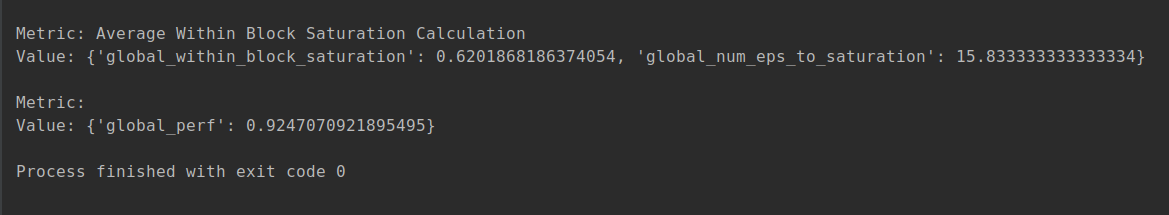
\includegraphics[width=0.85\columnwidth]{sections/figs/calc_metrics_output.png}
	\caption{Sample output for the example calc\_metrics.py .}
	\label{fig:calcmetricsoutput}
\end{figure}

Then, you should be able to:\\[0.1in]


5. Pass "YOUR\_LOG\_DIRECTORY" as the log\_dir parameter in the calc\_metrics.py file, and you should get an output printed to console that looks something like this: 


\begin{figure}[h]
	\centering
	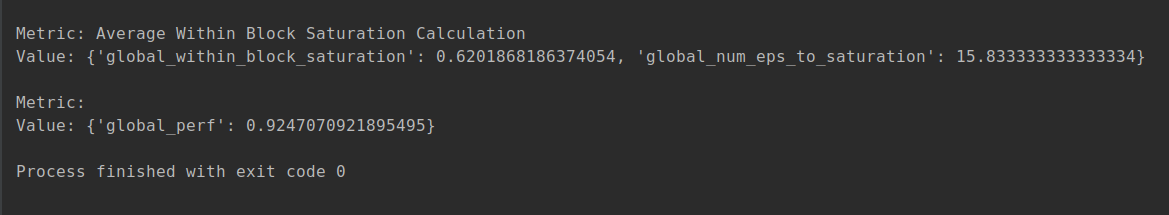
\includegraphics[width=0.85\columnwidth]{sections/figs/calc_metrics_output.png}
	\caption{Sample output for the example calc\_metrics.py .}
	\label{fig:calcmetricsoutput}
\end{figure}

\chapter{Creating Tasks Compatible with the Metrics Framework}\label{ch:task_design}

\section{Conceptual Overview}

\section{Sample Workflow - Connect Your Task Into the Metrics Framework}

\textit{Please note:} Log files should be generated automatically and should require no action on the performer's part. However, Single Task Expert JSON files and/or custom syllabi creation rules must be followed or the L2Metrics code may not work.\\[0.1in]

Log files \textbf{must} include logged reward, and the column in the data file \textbf{must} be named reward. Without this column, the metrics code will fail. This is assumed to be logged per episode. \\[0.1in]


\end{document}
